\section{Introduction}
Developing ``good'' mathematical models for representing basic motion skills continues to be a central focus in the literature on learning from demonstration~\cite{argall2009survey, saveriano2021dynamic, zhu2018robot}. In this paper, we adopt the view that a good model should be capable of generating diverse trajectories that can complete the given task. Moreover, it should be easily adaptable to a new, unseen constraint. For instance, if an unseen obstacle blocks the initially planned path, the model should enable a robot to avoid that obstacle while still accomplishing the task. We aim to train such a model using multiple demonstration trajectories. Challenges often arise from the small dataset size, high dimensionality of the trajectory data, and the multi-modality of data distribution.

Adopting the motion manifold hypothesis~\cite{arvanitidis2017latent, lee2023geometric} -- which assumes that a set of high dimensional trajectory data lies on some lower-dimensional manifold --, recent {\it Motion Manifold Primitives (MMP)} framework provides motion primitive models that can encode and generate, for a given task, a continuous manifold of trajectories each of which is capable of accomplishing the task~\cite{noseworthy2020task, lee2023equivariant}. 
This framework has demonstrated promising results in addressing the aforementioned challenges, effectively reducing the data dimensionality and capturing multi-modality. 
In particular, adjusting the low-dimensional latent coordinate values enables the adaptation of trajectories to unseen environments.

\begin{figure}[!t]
    \centering
    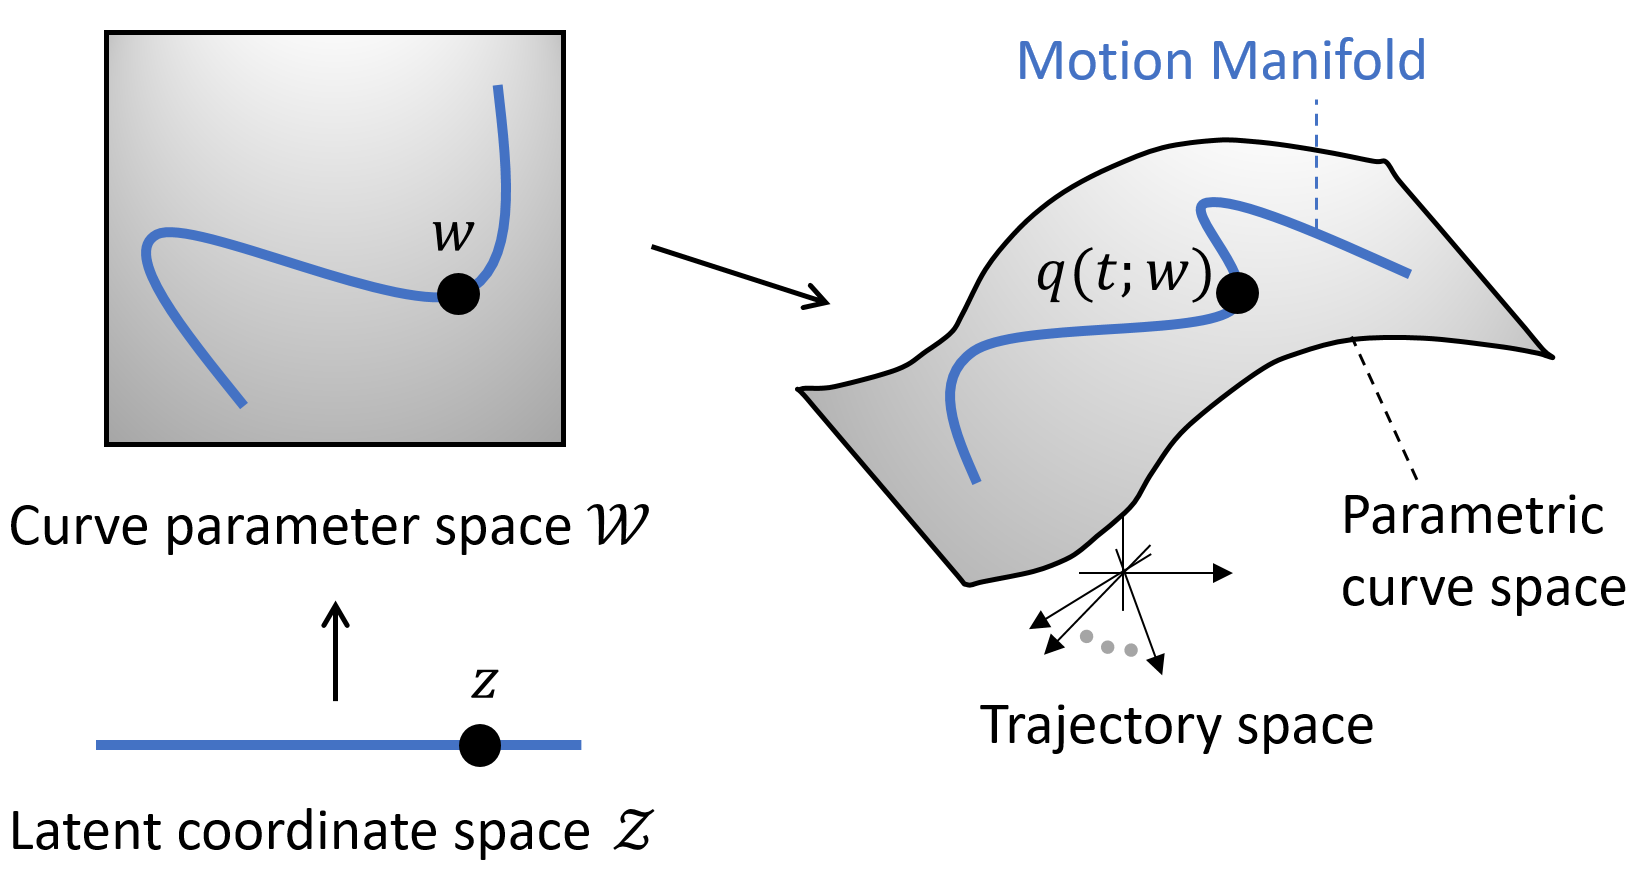
\includegraphics[width=0.9\linewidth]{figure/intro2.png}
    \caption{{\it MMP++}: A latent coordinate space ${\cal Z}$ is mapped to a subspace of the curve parameter space ${\cal W}$; the parameter space ${\cal W}$ is mapped to a subspace of the infinite-dimensional trajectory space.
    The motion manifold and parametric curve space are visualized as a curve and surface, not because their actual dimensions are one and two, but only to indicate the relative size relationships of their dimensions.} 
    \label{fig:intro2}
    \vspace{-5pt}
\end{figure}

These manifold-based models, however, lack some of the desired functionalities of movement primitives found in other conventional methods such as DMP~\cite{schaal2007dynamics, ijspeert2013dynamical}, ProMP~\cite{paraschos2013probabilistic}, and VMP~\cite{zhou2019learning}. These functionalities include: (i) temporal modulation to enable faster or slower execution of the movement and (ii) modulation of via-points (e.g., start and goal points) given new task constraints.
The fundamental reason for the absence of such functions in the MMP framework is its reliance on discrete-time trajectory representations.
In contrast, conventional movement primitives often employ parametric models for trajectory representation. For example, one of the simplest forms of these models is the linear basis function model, for a configuration space ${\cal Q}=\mathbb{R}^{n}$, expressed as:
\begin{equation}
    q(\tau; w) = \sum_{i=1}^{B} \phi_i(\tau) w_i \:\:\: \text{for} \:\:\: \tau \in [0,1],
\end{equation}
where $\{\phi_i(\tau)\}_{i=1}^{B}$ is a set of some scalar-valued basis functions in $[0,1]$ and $w_i \in \mathbb{R}^{n}, i=1,\ldots,B$ are curve parameters. 
Temporal modulation can be achieved by modifying $\tau$ as a function of time $t$, and adding some structures to the basis function $\phi_i(\tau)$ can enforce constraint satisfaction (e.g., $\phi_i(\tau):=\tau (1-\tau) b_i(\tau)$ enforces $\phi_i(0)=\phi_i(1)=0$ for any function $b_i(\tau)$).


In this paper, we propose applying the MMP framework to the parametric curve representations of trajectories, thus simultaneously tackling the challenge of dimensionality and achieving the desired functionalities, denoted as {\it MMP++} (see Fig.~\ref{fig:intro2}). 
Additionally, parametric curve representations in MMP++ lead to several other advantages. First, motions have bounded accelerations and jerks, avoiding sudden and abrupt changes. Second, the dimension of the parametric curve space -- which is equal to the dimension of the parameter space -- is generally much smaller than the dimension of the discrete-time trajectory data space, reducing the complexity of the subsequent motion manifold learning problem.

\begin{figure*}[!t]
    \centering
    
\includegraphics[width=1\textwidth]{figure/intro.png}
    \caption{\textit{Left}: There are 15 demonstration trajectories (red, green, and blue trajectories) that travel from the start to the goal, avoiding the obstacle. \textit{Middle and Right}: MMP++ and IMMP++ learn two-dimensional manifolds in the curve parameter space and produce two-dimensional latent coordinate spaces. Latent values of the demonstration trajectories are visualized in the latent coordinate spaces, marked as $\times$. GMMs of three components are fitted in the latent spaces, and the sampled points are visualized as stars $*$. The corresponding generated trajectories are also visualized.} 
    \label{fig:intro}
    \vspace{-5pt}
\end{figure*}

% Nevertheless, current parametric curve model-based methods continue to face challenges stemming from the high-dimensionality of the parameter space, resulting in less-than-desirable performance, as we show later in our experiments. 
% Although the parameter space has a lower dimension than the trajectory space, it is still not sufficiently low to enable accurate learning of movement primitives.
% To address this, we propose applying the MMP framework to the parametric curve representations of trajectories, thus simultaneously tackling the challenge of dimensionality and achieving the desired functionalities, denoted as {\it MMP++} (see Fig.~\ref{fig:intro2}).

The vanilla MMP++, a naive application of the MMP framework to the curve parameter space, however, sometimes results in a {\it geometrically distorted} latent coordinate space -- where similar motion data are not positioned close to each other --, leading to a generation of motions that violate the task constraint. 
For example, consider an example shown in Fig.~\ref{fig:intro}.
We learn a two-dimensional manifold and its latent coordinate space, by using the red, green, and blue demonstration trajectories and their parametric curve representations. 
Then we fit a Gaussian Mixture Model (GMM) using the latent values of the trajectories.
As illustrated in Fig.~\ref{fig:intro} (\textit{Middle}), due to the geometric distortion in the latent coordinate space, the same color trajectories are not located close enough to each other. Consequently, the red and green latent points are not correctly clustered by the GMM, and many of the generated motions collide with the obstacle, failing to accomplish the task.  
  

In this paper, adopting the isometric regularization method from~\cite{yonghyeon2022regularized}, we propose to learn {\it a geometry-preserving latent coordinate space}, so that similar trajectories can be located nearby in the latent space. 
To employ this method in our context, we need to specify a {\it Riemannian metric} for the curve parameter space that serves as the basis for determining the notion of closeness in the parameter space. 
We propose a {\it CurveGeom Riemannian metric} for the curve parameter space, that reflects the geometry of the trajectory space, given a parametric curve model that satisfies some mild regularity conditions.
We call this framework {\it Isometric Motion Manifold Primitives++ (IMMP++)}; see Fig.~\ref{fig:intro} ({\it Right}).

In the first part of our experiments, we focus on Euclidean configuration space cases and use affine curve models, similar to those in ProMP~\cite{paraschos2013probabilistic} and VMP~\cite{zhou2019learning}. This induces constant CurveGeom metrics and leads to simpler implementations of the isometric regularization. Experiments involving 2-DoF planar obstacle-avoiding motions and 7-DoF collision-free motions of a robot arm confirm that our manifold-based methods, MMP++ and IMMP++, outperform conventional movement primitives in trajectory generation. Notably, we verify that the modulation of latent coordinates and via-points leads to diverse trajectory generation and enables the online adaptation of trajectories in dynamic environments.  In the second part, we demonstrate how to extend our framework to SE(3) trajectory data with the water-pouring demonstration trajectory dataset.